\let\negmedspace\undefined
\let\negthickspace\undefined
\documentclass[journal]{IEEEtran}
\usepackage[a5paper, margin=10mm, onecolumn]{geometry}
%\usepackage{lmodern} % Ensure lmodern is loaded for pdflatex
\usepackage{tfrupee} % Include tfrupee package

\setlength{\headheight}{1cm} % Set the height of the header box
\setlength{\headsep}{0mm}     % Set the distance between the header box and the top of the text

\usepackage{gvv-book}
\usepackage{gvv}
\usepackage{cite}
\usepackage{amsmath,amssymb,amsfonts,amsthm}
\usepackage{algorithmic}
\usepackage{graphicx}
\usepackage{textcomp}
\usepackage{xcolor}
\usepackage{txfonts}
\usepackage{listings}
\usepackage{enumitem}
\usepackage{mathtools}
\usepackage{gensymb}
\usepackage{comment}
\usepackage[breaklinks=true]{hyperref}
\usepackage{tkz-euclide} 
\usepackage{listings}
% \usepackage{gvv}                                        
\def\inputGnumericTable{}                                 
\usepackage[latin1]{inputenc}                                
\usepackage{color}                                            
\usepackage{array}                                            
\usepackage{longtable}                                       
\usepackage{calc}                                             
\usepackage{multirow} 
\usepackage{hhline}                                           
\usepackage{ifthen}                                           
\usepackage{lscape}
\usepackage{circuitikz}
\tikzstyle{block} = [rectangle, draw, fill=blue!20, 
    text width=4em, text centered, rounded corners, minimum height=3em]
\tikzstyle{sum} = [draw, fill=blue!10, circle, minimum size=1cm, node distance=1.5cm]
\tikzstyle{input} = [coordinate]
\tikzstyle{output} = [coordinate]

\begin{document}
\bibliographystyle{IEEEtran}
\vspace{3cm}

\title{MatGeo Assignment 8.2.43}
\author{AI25BTECH11007}
 \maketitle
% \newpage
% \bigskip
{\let\newpage\relax\maketitle}

\renewcommand{\thefigure}{\theenumi}
\renewcommand{\thetable}{\theenumi}
\setlength{\intextsep}{10pt} % Space between text and floats


\numberwithin{equation}{enumi}
\numberwithin{figure}{enumi}
\renewcommand{\thetable}{\theenumi}
\noindent
\textbf{Question :}\\
Find the equation of the conic, that satisfies the given conditions. \\ 
Focus at (-1, 2), directrix x - 2y + 3 =  0.  

\noindent\\
\textbf{Solution :}\\
Let :
\begin{align}
    \vec{F} &= \myvec{-1\\2}\\[4pt]
    \text{directrix equation is :} \quad &x - 2y + 3 = 0 
    \quad\Longrightarrow\quad \myvec{1\\-2}^{T}\vec{x} = -3
\end{align}
The equation of a conic with directrix $\vec{n}^{T}\vec{x} = c$, eccentricity $e$ and focus $\vec{F}$ is given by:
\begin{align}
    g(\vec{x}) = \vec{x}^{T}\vec{V}\vec{x} + 2\vec{u}^{T}\vec{x} + f  = 0
\end{align}

where :
\begin{align*}
\vec{V} &= \lVert \vec{n} \rVert^{2}\vec{I} - e^{2}\vec{n}\vec{n}^{T} , \\
\vec{u} &= ce^{2}\vec{n} - \lVert \vec{n} \rVert^{2}\vec{F} , \\
f &= \lVert \vec{n} \rVert^{2}\lVert \vec{F} \rVert^{2} - c^{2}e^{2}
\end{align*}

From the question we can say that the conic is a parabola so $e = 1$.\\
Calculating $\vec{V}$, $\vec{u}$ and $f$ by using the above equations we get :

\[
\vec{n}=\myvec{1\\-2},\qquad \|\vec{n}\|^2=5,\qquad c=-3,\qquad \|\vec{F}\|^2=5
\]

\begin{align}
   \vec{V} &= 5\vec{I} - \vec{n}\vec{n}^T
   = \myvec{4 & 2\\[2pt] 2 & 1}\\[6pt]
   \vec{u} &= c\vec{n} - 5\vec{F}
   = \myvec{2\\-4}\\[6pt]
   f &= 5\cdot 5 - (-3)^2 = 16
\end{align}

Finding eigen values of $\vec{V}$ :
\begin{align}
    \det\lvert \vec{V} - \lambda\vec{I} \rvert &= 0\\[4pt]
    \det\begin{pmatrix} 4 - \lambda & 2 \\[2pt] 2 & 1 - \lambda \end{pmatrix} &= 0\\[4pt]
    \lambda &= 5 \quad \text{and} \quad 0
\end{align}

Eigen vectors $\vec{v}$ for any square matrix $\vec{A}$ are defined by:
\begin{align}
    \vec{A}\vec{v} = \lambda\vec{v}
\end{align}
For $\lambda = 0$ and $\lambda=5$ we get
\begin{align}
    \lambda = 0 &\quad\Rightarrow\quad \vec{v}_1 = \myvec{1\\-2},\\[4pt]
    \lambda = 5 &\quad\Rightarrow\quad \vec{v}_2 = \myvec{2\\1}.
\end{align}

Substituting in the equation (0.3) we get the equation of the conic to be :
\begin{align}
  \vec{x}^{T}\myvec{4 & 2\\[2pt] 2 & 1}\vec{x} + 2\myvec{2 & -4}\vec{x} +16 =0
\end{align}

\begin{figure}[H]
    \centering
    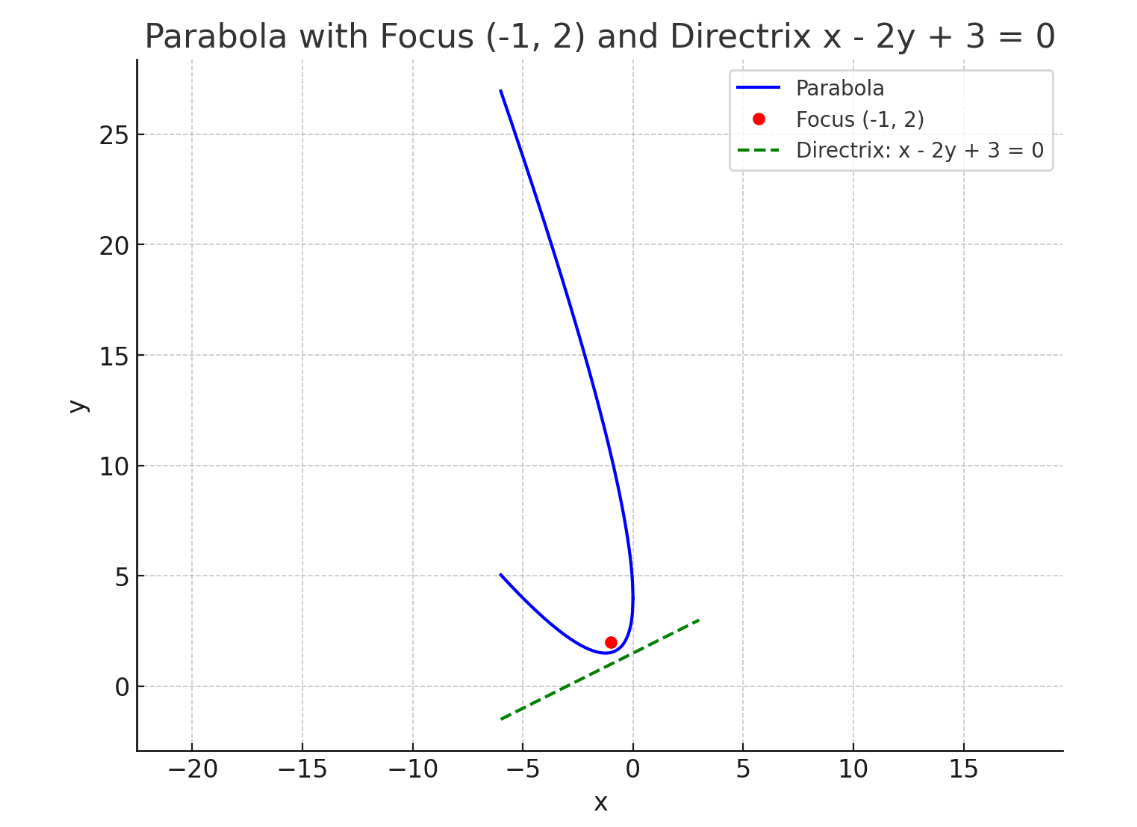
\includegraphics[width=0.85\linewidth]{figs/image.png}
    \caption{Image}
    \label{fig:placeholder}
\end{figure}
\end{document}